\chapter{\textbf{METODOLOGIA}}
\label{metodologia}

A metodologia utilizada no projeto é a exploratória.

Segundo \citeonline{VENTURA2007}, são verificadas grandes utilidades em estudos de casos realizados através de pesquisas exploratórias.

\begin{citacao}
“Por sua flexibilidade, é recomendável nas fases iniciais de uma investigação sobre temas complexos, para a construção de hipóteses ou reformulação do problema. Também se aplica com pertinência nas situações em que o objeto de estudo já é suficientemente conhecido a ponto de ser enquadrado em determinado tipo ideal. São úteis também na exploração de novos processos ou comportamentos, novas descobertas, porque têm a importante função de gerar hipóteses e construir teorias. Ou ainda, pelo fato de explorar casos atípicos ou extremos para melhor compreender os processos típicos \cite{VENTURA2007}.”
\end{citacao}

Sendo assim, será feito um estudo bibliográfico a partir do tema de visão computacional utilizando o acervo disponível sobre o assunto, com a finalidade de reunir informações para obter melhores resultados.

A pesquisa qualitativa será baseada principalmente nos três livros escolhidos: \textit{Digital Image Processing} \cite{GONZALEZ2002},  \textit{Computer Vision: Algorithms and Applications} \cite{SZELISKI2010} e Processamento Digital de Imagens \cite{FILHO1999}. Todos os livros foram escolhidos por transmitirem conceitos científicos, didáticos, teóricos e práticos sobre o assunto de visão computacional.

O desenvolvimento da aplicação proposta será feito através de estudos realizados sobre o tema. A aplicação será desenvolvida utilizando metodologia de desenvolvimento ágil, ou seja, será feita o planejamento de cada etapa de desenvolvimento do sistema, na qual o objetivo de cada entrega é proporcionar uma prévia do funcionamento do \textit{software}. Essa ação foi tomada para que a evolução do sistema seja gradativa e eficiente.

Para resumir as etapas desta pesquisa, foi elaborado uma imagem ilustrativa da metodologia utilizada no decorrer do desenvolvimento deste projeto (\autoref{fig_metodologia-desenvolvimento-tcc}).

\begin{figure}[h]
	\caption{\label{fig_metodologia-desenvolvimento-tcc}Metodologia de desenvolvimento do projeto.}
	\begin{center}
		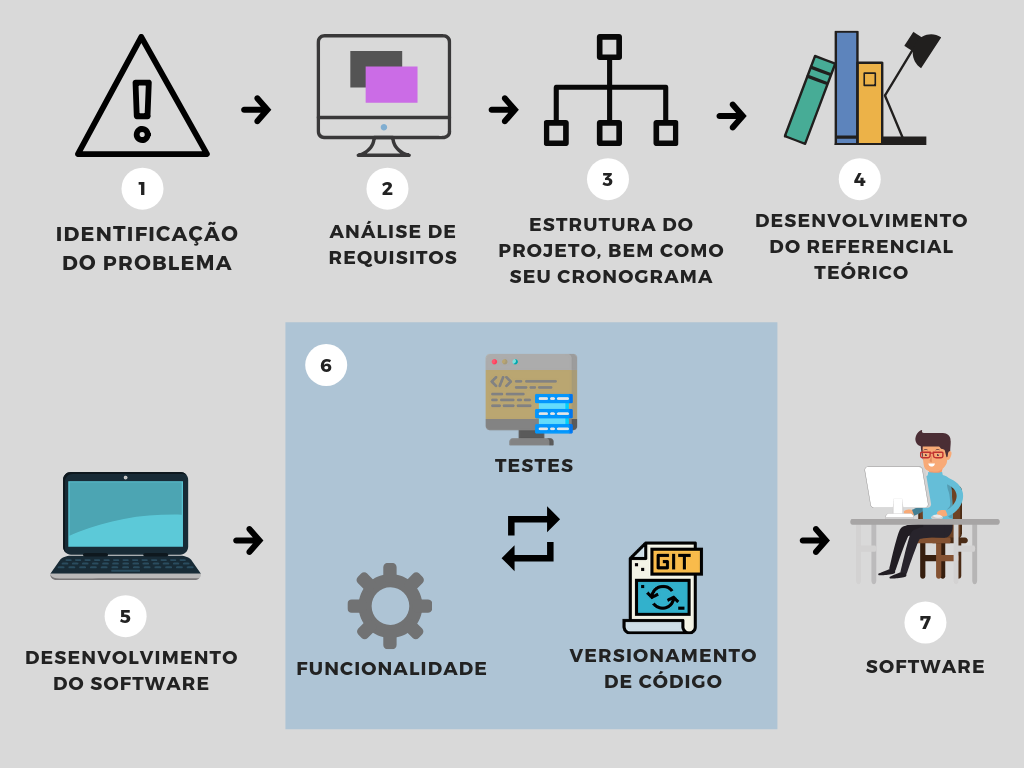
\includegraphics[scale=0.5]{5-Metodologia/metodologia-desenvolvimento-tcc.png}
	\end{center}
	\centering \legend{Fonte: Elaborada pelos autores.}
\end{figure}